\Jose{In this section I'll use the same notation used in \cite{Navarro:2014:FFS:2620785.2601073}. This notation should be introduced in the Related Work section}\\

\subsection{Parallel Succinct Tree Algorithm}

We propose a parallel algorithm based in the construct of the \emph{Range Min-Max Tree}, {\tt RMMT}\cite{Navarro:2014:FFS:2620785.2601073}. Our algorithm, called \emph{Parallel Succinct Tree Algorithm}, {\tt PSTA}, has as input a possibly non-balanced parentheses sequence $P$, where an opened-parenthesis is encoded by \emph{1} and a closed-parenthesis by \emph{0}.

The {\tt RMMT} is constructed over $P$, partitioning $P$ in disjoint chunks of size $s$. Considering those chunks, the construction of the {\tt RMMT} is based in the computation of different arrays of size $O(\frac{n}{s})$. Such arrays are $e^{\prime}$, saving the final excess of each chunk, $m^{\prime}$, saving the minimum excess value of each chunk, $M^{\prime}$, saving the maximum excess value of each chunk and $n^{\prime}$, saving the number of ocurrences of the minimum value of each chunk. As a reminder, the excess value at position $i$ is:
	\begin{center}
		$\displaystyle E[i] = \sum_{k=0}^{i} \pi(P[k])$	
	\end{center}

where $\pi(``(") = 1$ and $\pi(``)") = -1$. See Figure \ref{fig:RangeMinMaxTree} as an example of {\tt RMMT}.

 	\begin{figure}[ht]
		\centering
		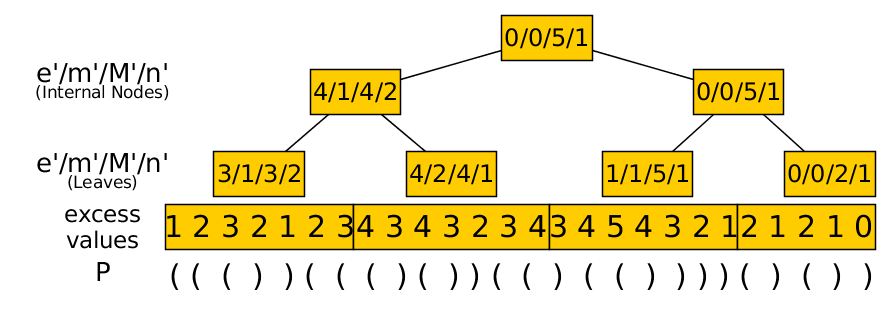
\includegraphics[scale=0.13]{./images/Range-min-max-tree.png}
     	\caption{Range min-max tree}
		\label{fig:RangeMinMaxTree} 
	\end{figure}

The first step of {\tt PSTA} is to compute the arrays $e^{\prime}$, $m^{\prime}$, $M^{\prime}$ and $n^{\prime}$ in parallel. Since $e^{\prime}$ just saves the last excess value of each chunk, which is a sum, {\tt PSTA} needs to apply a parallel list-ranking algorithm. Computing the last element of $e^{\prime}$, at position $\frac{n}{s}-1$, we indirectly compute the rest of the elements of $e^{\prime}$. We adapted the algorithm in \cite{Helman2001265} for this context, computing $e^{\prime}$ in $O(\frac{n}{p})$ time, using $p$ threads. Note that we do not need to compute more elements of $e^{\prime}$ to the internal nodes of the {\tt RMMT}. The final size of $e^{\prime}$  and the memory used in construction time are bounded by $O(\frac{nc\lg(w)}{w})$ bits, where $c\geqslant 1$ and $w$ is the word size in the RAM model.

To compute $m^{\prime}$, let's assume, without loss of generality, that $p = k^{i}$, where $k = \Theta(\frac{w}{c\lg(w)})$ is the arity of the vertices in the {\tt RMMT} and $i > 0$. {\tt PSTA} assigns one thread per sub-tree of size $O(\frac{n}{sp})$, at level $i$. So, it is possible to compute the $m^{\prime}$ values in all sub-trees, in parallel, in $O(\frac{n}{sp}k)$ time. Then, for the rest $O(p)$ vertices in the top of the tree, we compute the corresponding minimum values in $O(k\lg_{k} p)$ time, computing each level in $O(k)$ time, just looking the $k$ values on the previous level using one thread per vertex. If we consider $k$ has a constant, we can compute $m^{\prime}$ in $O(\frac{n}{sp}k + \lg p) = O(\frac{n}{p\lg(w)}+\lg p)$ time, using $O(\frac{nc\lg(w)}{w})$ bits in construction time and in the final array. Note that this solution makes sense considering that $p\ll n$. Figure \ref{fig:min-max-array} illustrates the solution explained here. We can compute $M^{\prime}$ and $n^{\prime}$ in the same way, obtaining the same complexities.

	 	\begin{figure}[ht]
			\centering
			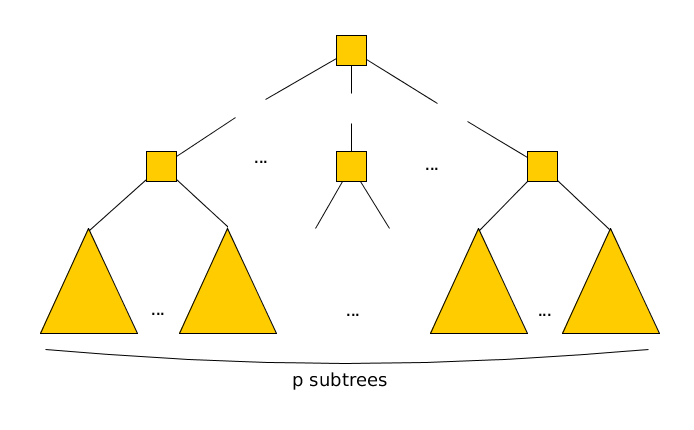
\includegraphics[scale=0.28]{./images/Min-Max-array.png}
     		\caption{Computation of $m^{\prime}$ and $M^{\prime}$}
			\label{fig:min-max-array} 
		\end{figure}

	\Jose{In construction}

\subsection{Theoretical Analysis}

	\Jose{In construction}
